%The following section describes how the tests were set up and carried out.
%
%\subsubsection{Experimental Setup}
The tests were carried out using an optical bench to guarantee scientific accuracy, with a screen holder at the zero point, where the QR code was positioned. The device being tested, Google Glass or a smartphone, was then positioned at the specified mark on the optical bench, using a clamp, and pointed towards the QR code. See Figure~\ref{experimentalSetup} for a better understanding of the experimental setup. 

As seen in Figure~\ref{experimentalSetup} Google Glass was mounted in such a way that the camera sat a bit closer to the QR code than where the clamp marked on the optical bench. In order to compensate for the slight misalignment the clamp was positioned a few centimeters back from the specified mark and as such not used to determine the distance to the QR code. Instead the camera on Google Glass was used to pinpoint the exact distance to the QR code, and the clamp was positioned in such a way that the camera on Google Glass was at the distance specified in each experiment. In other words, even though the clamp was not at the same distance to the QR code for the smartphone tests as for the Google Glass tests, the camera of each device was.

	\begin{figure}[H]%ht!]
		\centering
    		\subfloat[The experimental setup for Google Glass.]{{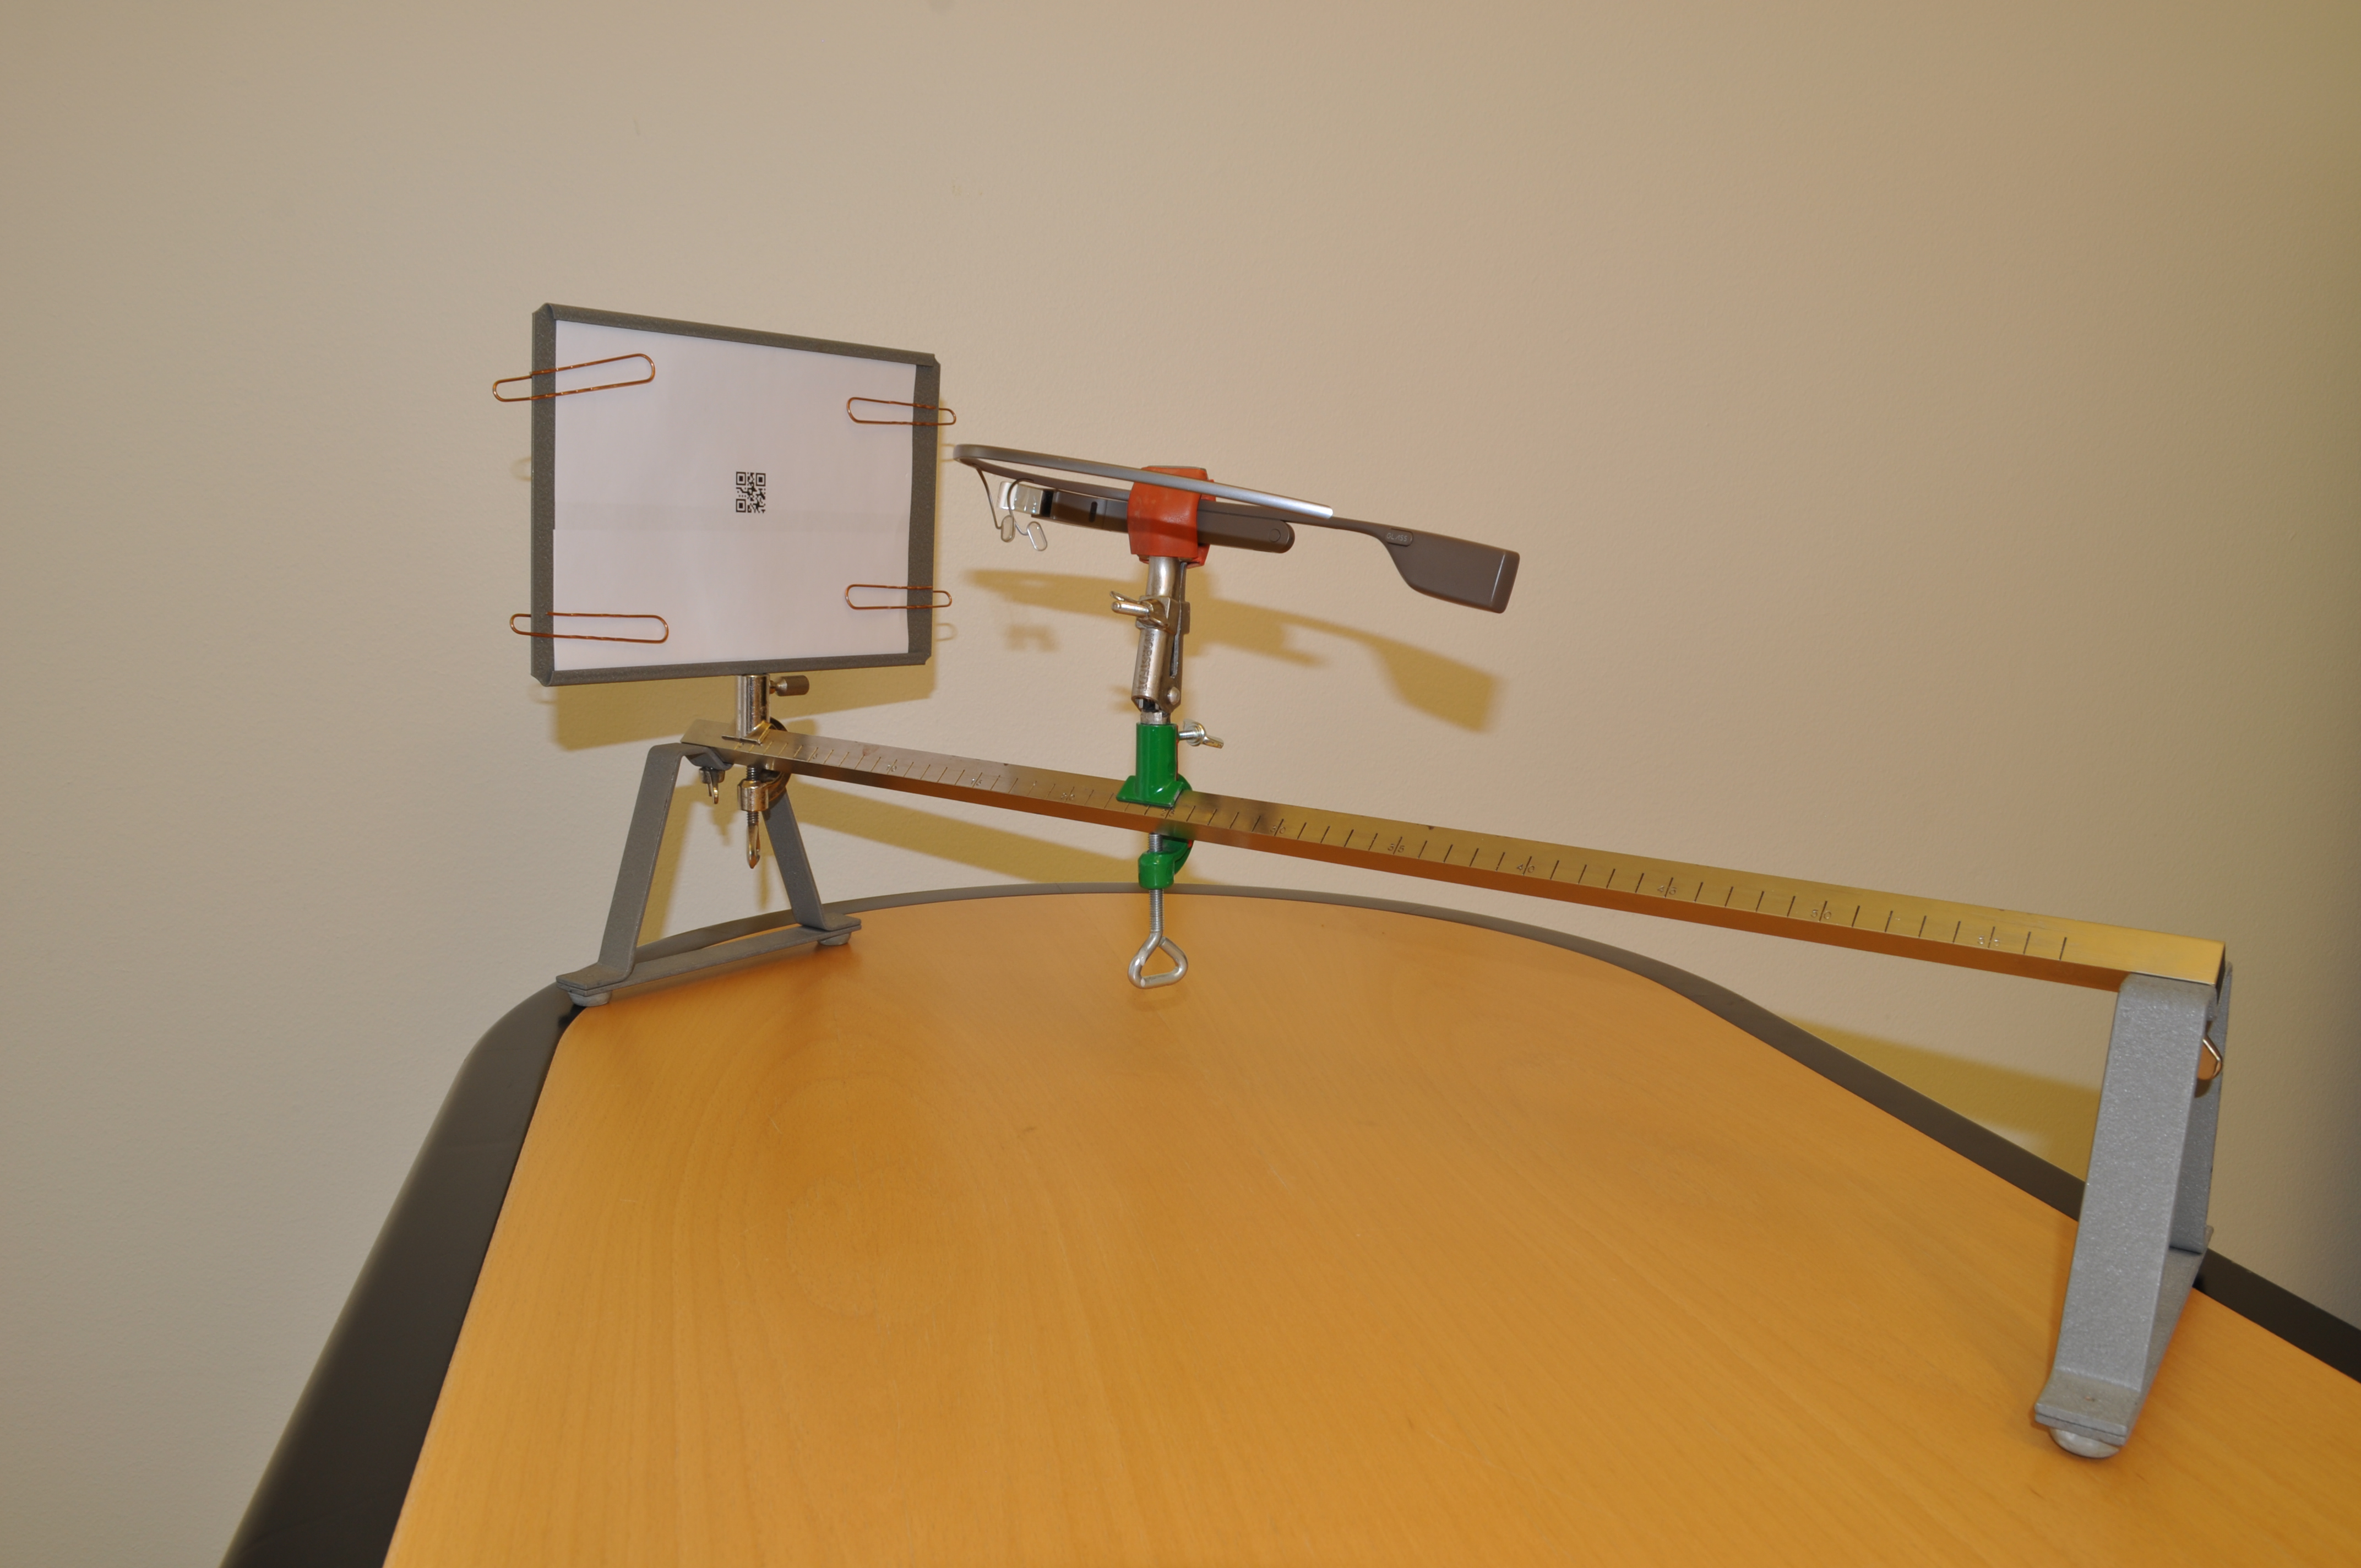
\includegraphics[width=70mm]{images/testSetupGlass}}}
   		 \qquad
		\subfloat[The experimental setup for the Samsung Galaxy SII.]{{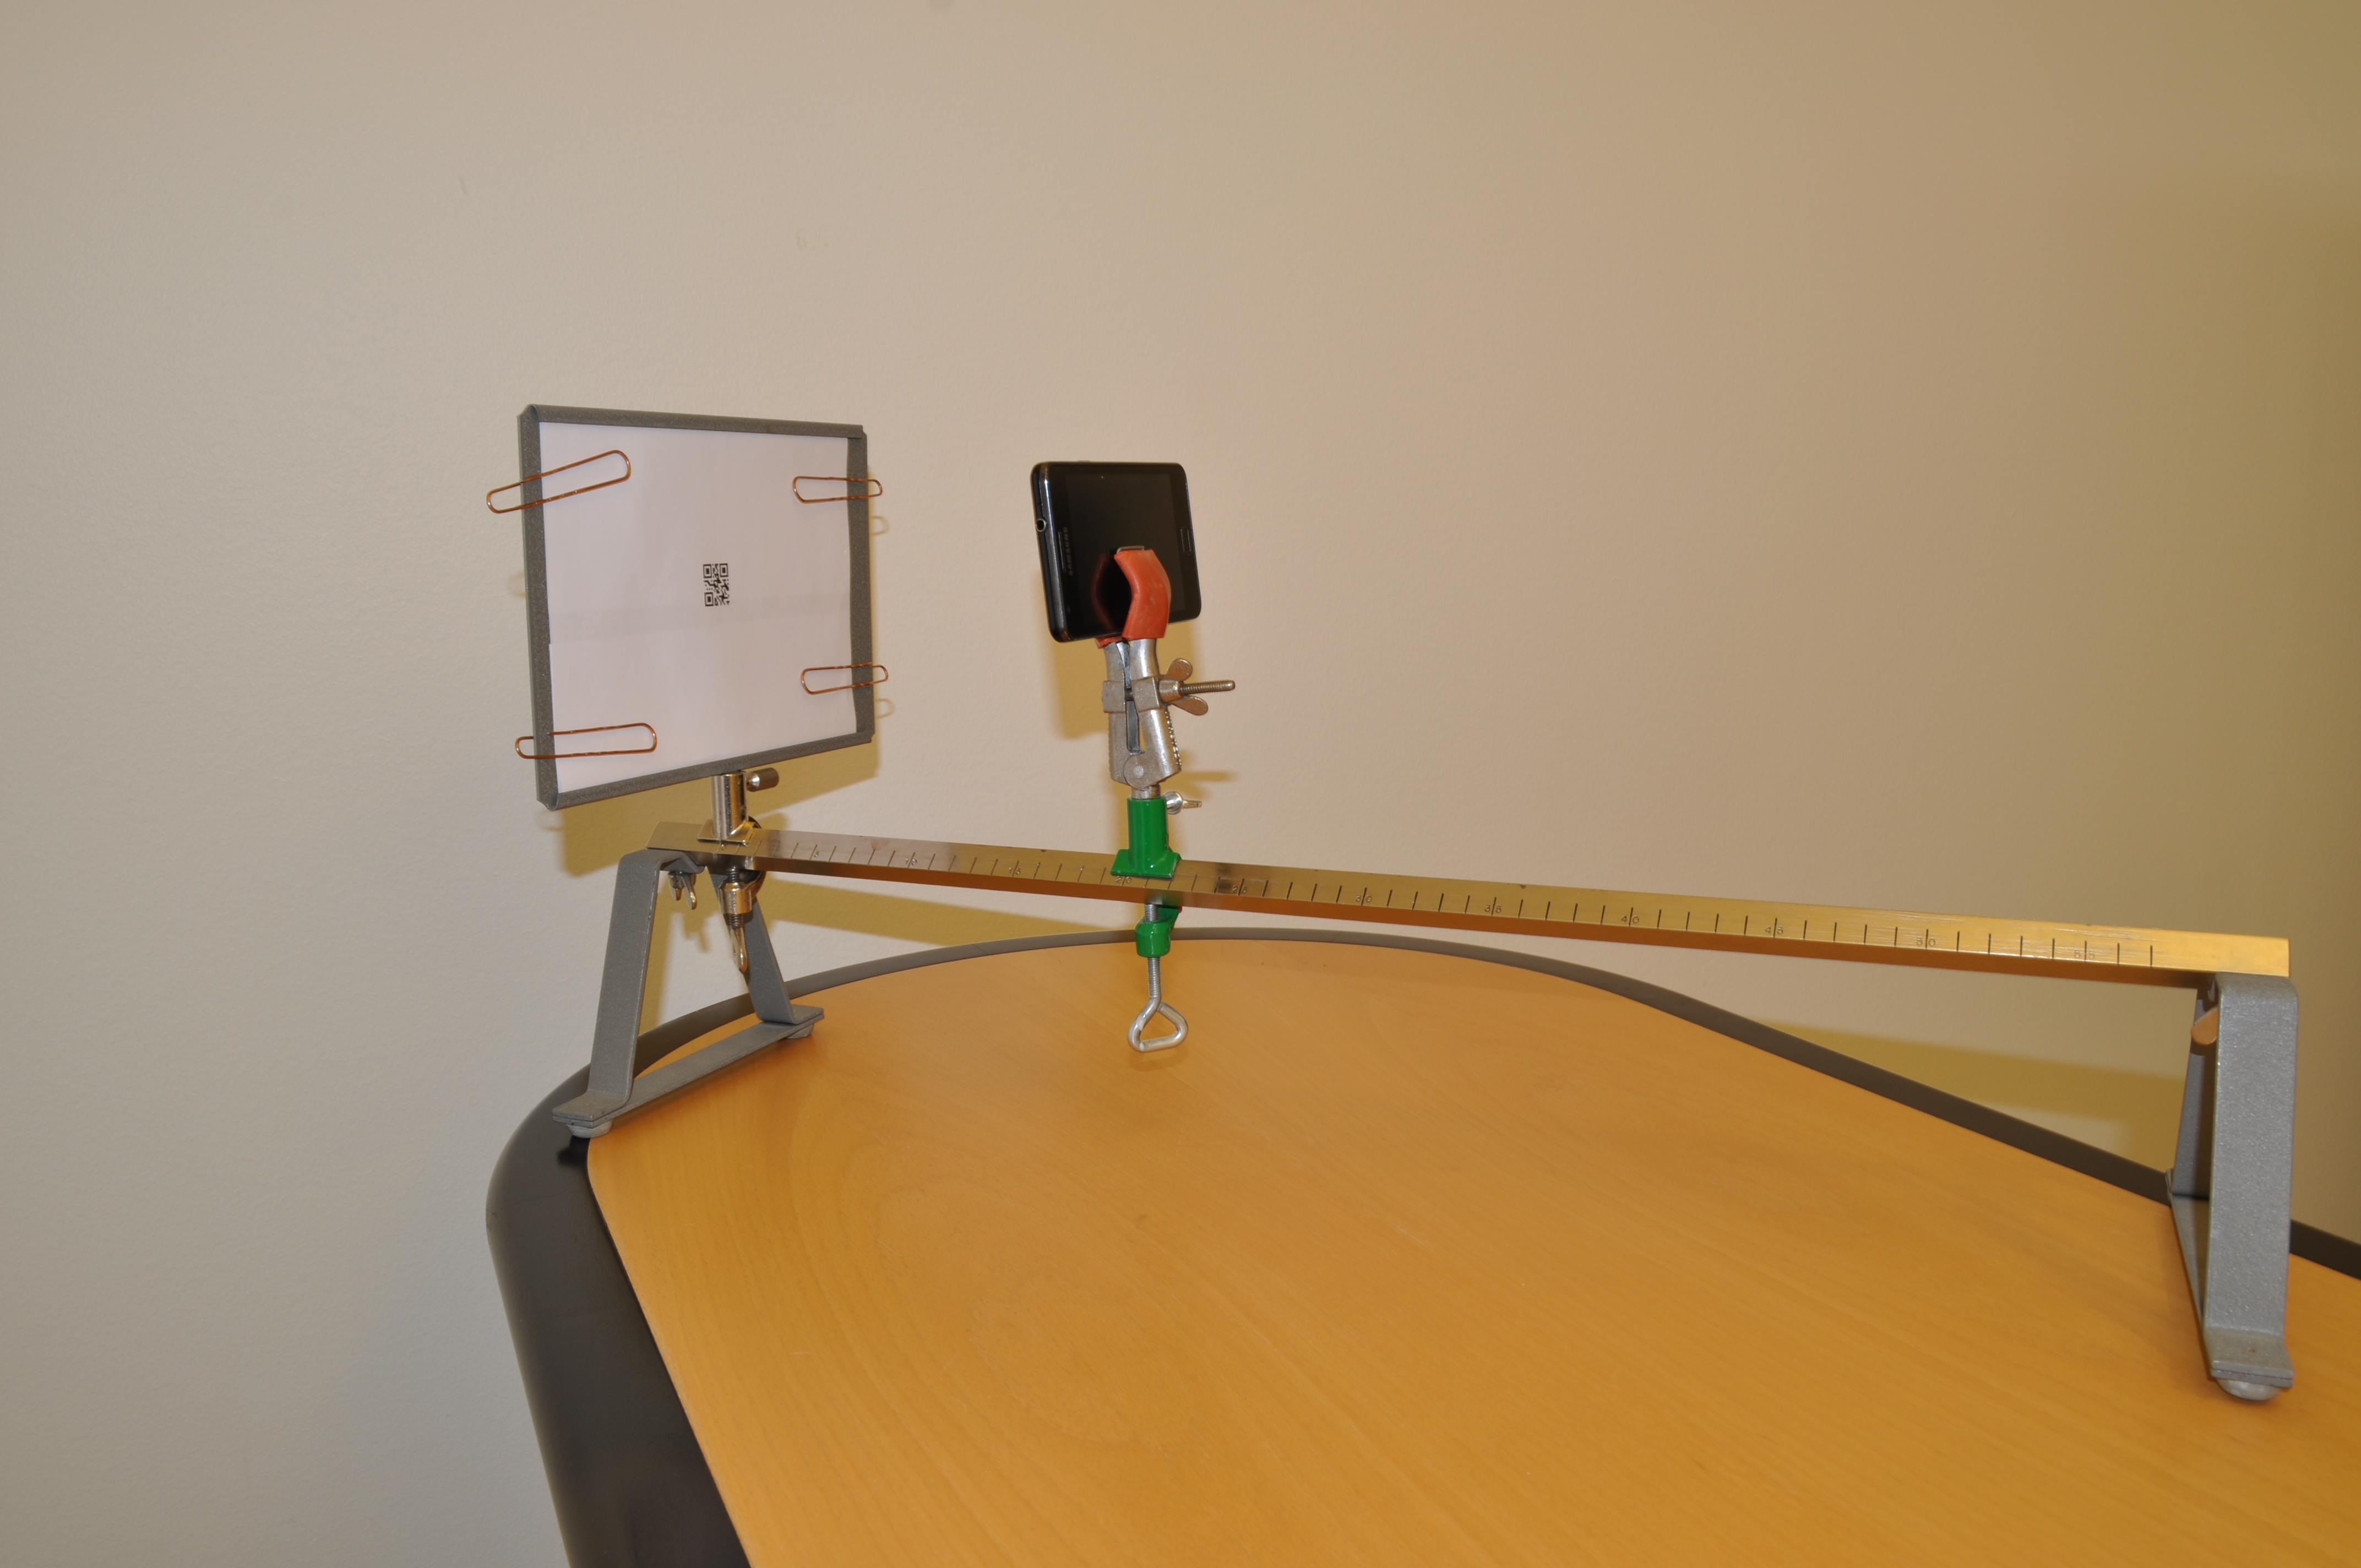
\includegraphics[width=70mm]{images/testSetupS2}}}
   		 \qquad
		\caption{The experimental setup.}
		\label{experimentalSetup}
	\end{figure}

Although not shown i Figure~\ref{experimentalSetup}, each device was connected to a computer via a USB cable. The result time of each test was obtained from the log within Android Studio after each run, since when running an android application via Android Studio, log information may be obtained through the log within Android Studio.

In order to measure the time needed for the results of each test a specific class was built, called \texttt{Timer} (seen in Listing~\ref{timerClass}). The \texttt{Timer} class was built using the singleton design pattern. A singleton class is a class that can only be instanced once during the entire execution of an application. However, the instance of a singleton class lives throughout the entire execution and may be accessed from anywhere in the application~\cite{singleton}.

Using the singleton pattern meant that the timer could be started in one class, and stopped in another, without having to pass the instance around, potentially affecting the performance of each device.
\newpage
\begin{lstlisting}[language=Java, caption={The Timer class}, label=timerClass]

public class Timer {
	private static Timer ourInstance = new Timer();
	public static Timer getInstance() { return ourInstance; }
	private Timer() {  }
	
	private boolean timerRunning = false;
	private Long startTime;
	private Long stopTime;
	
	public void startTimer() { 
		if(timerRunning) { Log.d("TIMER", "Timer already running"); }
		else 	{ startIme = System.nanoTime(); }
	}
	
	public void stopTimer() {
		if(!timerRunning) { Log.d("TIMER", "No timer running"); }
		else { stopTime = System.nanoTime()); }
	}
	
	private long getElapsedTime(int timerID) { return stopTime - startTime; }
	
	public void logElapsedTime(String information) {
		Log.d("TIMER", information + ": " + String.valueOf(getElapsedTime() + " nano seconds");
	}
}
\end{lstlisting}

\subsubsection{Text Length}
When evaluating the text length, the text string used was not a predefined string, but rather a randomised string. The text was randomly generated using the distribution of characters in regular English text. One might argue that technical texts have a slightly different distribution of characters, but Google recommends developers to be personal when writing text meant to be displayed to the user~\cite{glassDesignStyle}. The text was also short enough to fit a smartphone screen and as such the difference using slightly different distribution of characters would not have any major effect on the results.

Listing~\ref{randomizer} shows how each character was randomly selected. \texttt{randchar} was called from within a for loop, where the character was added to a string. The number of loops determined how long the text was going to be. The \texttt{doubleList} list contained the distribution of each character according the their distribution in the english language~\cite{englishTextStat}, and the \texttt{alph} list contained all the individual characters, including whitespace. As a decimal number between zero and one was randomly selected, a corresponding character was picked out based on the distribution of that character.

A recursive method located the corresponding character and returned the character back up to the calling method \texttt{randchar}, which in turns returned the character to the for loop in which a string of random characters were collected.

\newpage
\begin{lstlisting}[language=Java, caption={The randomizer class}, label=randomizer]
public RandomizeEnglishText() {
	doubleList = new ArrayList<>();
	doubleList.add(0.0651738);										// A
	doubleList.add(doubleList.get(0) + 0.0124248);		// B
	doubleList.add(doubleList.get(1) + 0.0217339);		// C
		[...]
	doubleList.add(doubleList.get(23) + 0.0145984);	// Y
	doubleList.add(doubleList.get(24) + 0.0007836);	// Z
	doubleList.add(doubleList.get(25) + 0.1918182);	// _
	alph = Arrays.asList("a", "b", "c", "d", "e", "f", "g", "h", "i", "j", "k", "k", "m", "n", "o", "p", "q", "r", "s", "t", "u", "v", "w", "x", "y", "z", " ");
}
private double randfrom(double min, double max) {
	Random rand = new Random();
	double range = (max - min);
	return min + range * rand.nextDouble();
}
private String getChar(int pos, double rand) {
	return (rand <= doubleList.get(pos) || pos+1 <= alph.size()) ?
		alph.get(pos) :
		getChar(pos+1, rand);
}
public String randchar() {
	double rand = randfrom(0, 1);
	return getChar(0, rand);
}
\end{lstlisting}

\subsubsection{Distance to the QR Code}

Using the \texttt{Timer} class, seen in Listing~\ref{timerClass}, the elapsed time from the start of the application until the QR code was decoded was measured for each device. The test was performed 30 times for each device, with 3 different distances between the QR code and the device. Figure~\ref{projectmap} described the application functionality and this test measures steps 1 and 2 in Figure~\ref{projectmap}.
%in a table similar to Table~\ref{tab:distanceAverage}. 

Although the \texttt{Timer} class will give the elapsed time in nanoseconds the result will be presented in seconds in order to clearly show the significance of each time as small, nano seconds, differences between devices will not matter as much as seconds.

%	\begin{table}[ht!]
% 		\caption{Average time of registering a QR code with varying distance.} \label{tab:distanceAverage}
%		\centering \begin{tabularx}{\textwidth}{l|X|X|X} \hline
%		\textbf{Distance (dm)} & \textbf{Google Glass (sec)} & \textbf{Samsung Galaxy SII (sec)} & \textbf{Samsung Galaxy SIII (sec)} \\ \hline \hline
%       
%		1.0	&	&	&	\\ \hline
%		2.0	&	&	&	\\ \hline
%		3.0	&	&	&	\\ \hline
%		
%		\end{tabularx}
%	\end{table}

\subsubsection{Complexity of the QR Code}

Using the \texttt{Timer} class, seen in Listing~\ref{timerClass}, the elapsed time from the start of the application until the QR code was decoded was measured for each device. The test was performed 30 times for each device, with 3 different complexities of the QR code. Figure~\ref{projectmap} described the application functionality and this test measures steps 1 and 2 in Figure~\ref{projectmap}.
% in a table similar to Table~\ref{tab:complexityAverage}. 

Although the \texttt{Timer} class will give the elapsed time in nano seconds the result will be presented in seconds in order to clearly show the significance of each time as small, nanoseconds, differences between devices will not matter as much as seconds. Figure~\ref{qrCodeComplex} shows the three different QR codes used for the complexity test.

	\begin{figure}[H]%ht!]
		\centering
    		\subfloat[1 encoded character.]{{
\includegraphics[width=20mm]{images/qrCodeComplex/1}}}
   		 \qquad
		\subfloat[50 encoded characters.]{{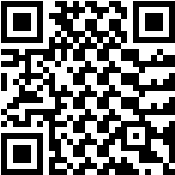
\includegraphics[width=20mm]{images/qrCodeComplex/50}}}
   		 \qquad
		\subfloat[100 encoded characters.]{{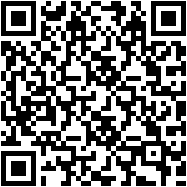
\includegraphics[width=20mm]{images/qrCodeComplex/100}}}
   		 \qquad
		\caption{The three different QR codes used in the complexity test.}
		\label{qrCodeComplex}
	\end{figure}

%	\begin{table}[H]%ht!]
%    		\caption{Average time of registering a QR code with varying density.} \label{tab:complexityAverage}
%		\centering \begin{tabularx}{\textwidth}{l|X|X|X} \hline
%		\textbf{Encoded Characters} & \textbf{Google Glass (sec)} & \textbf{Samsung Galaxy SII (sec)} & \textbf{Samsung Galaxy SIII (sec)} \\ \hline \hline
%       
%		1	&	&	&	\\ \hline
%		50	&	&	&	\\ \hline
%		100	&	&	&	\\ \hline
%		
%		\end{tabularx}
%	\end{table}

\subsubsection{Display Time}

Using the \texttt{Timer} class, seen in Listing~\ref{timerClass}, the elapsed time from the point that the product information had ben downloaded until the information was sent to the display was measured for each device. The test was performed 30 times for each device, with 3 different sizes of product information. Figure~\ref{projectmap} described the application functionality and this test measures steps 4 and 5 in Figure~\ref{projectmap}. %in a table similar to Table~\ref{tab:averageDisplaySpeedGoogleGlass}. 

Although the \texttt{Timer} class will give the elapsed time in nanoseconds the result will be presented in seconds in order to clearly show the significance of each time as small, nano seconds, differences between devices will not matter as much as seconds.

%	\begin{table}[ht!]
%    		\caption{Average display time for Google Glass with varying information size.} \label{tab:averageDisplaySpeedGoogleGlass}
%		\centering \begin{tabularx}{\textwidth}{l|X|X|X} \hline
%		\textbf{Information Size (Bytes)} & \textbf{Google Glass (sec)}  & \textbf{Samsung Galaxy SII (sec)}  & \textbf{Samsung Galaxy SIII (sec)} \\ \hline \hline
%       
%		1 000		&	&	&	 \\ \hline
%		100 000		&	&	&	 \\ \hline
%		1 000 000		&	&	&	 \\ \hline
%
%		\end{tabularx}
%	\end{table}